\documentclass[12pt]{article}
\usepackage[backend=biber]{biblatex}
\addbibresource{ProjectProp.bib}

\usepackage{graphicx} %intersting images
\usepackage{float} %for placement of images
\usepackage{lipsum} %fill
\usepackage{tocloft} %for dots on table of contents
\renewcommand{\cftsecleader}{\cftdotfill{\cftdotsep}}

\begin{document}

\begin{titlepage}
	\centering{
\includegraphics[scale=0.7]{ProjectPropFigure/BUlogo.jpg}\\
	\vspace{3em}
	\bfseries{\large{Department of Electrical and Computer Engineering}}\\
	\vspace{2em}
	\bfseries{\large{Senior Capstone Project Proposal}}\\
	\vspace{2em}
	\bfseries{\Large{Charge Pump}}\\
	\vspace{2em}
	\bfseries{\large{Authors: Derek Brissey \& John Clapham}}\\
	\textit{\large{Advisors: Dr. Brian Huggins \& Dr. Prasad Shastry}}\\
	\vspace{2em}
	\today
	}
\end{titlepage}

	\pagenumbering{roman}

	\begin{abstract}
Radio frequency~(RF) energy harvesting devices can be a useful battery alternative for low power applications such as periodic sensor measurements. A passive charge pump topology using Schottky diodes and capacitors can be implemented to step up the voltage of a low power RF input signal to a usable Direct Current~(DC) steady state. This capstone project will include research and simulation, design, and eventually populating a printed circuit board~(PCB) with specified components for testing. This project will explore how the variabilities in a charge pump design (such as number of stages, capacitor values, and a switching device) can be evaluated to produce a more efficient RF-DC conversion for specified frequencies. The exploration of this design will be conducted in frequencies less than 100kHz for analysis in the time domain with the hope to scale up to RF frequencies.
	\end{abstract}
	
	\newpage
	\tableofcontents
	\newpage
	
	\pagenumbering{arabic}
	
\section{Introduction}
Electromagnetic signals that oscillate in the range of 300MHz to 300GHz are known as Radio Frequency~(RF) waves. Due to the widespread use of RF signals, interest in harvesting the low transmitted energy has become a popular concept. This is known as RF energy harvesting. It is normally difficult to collect enough energy from these RF signals to be usable due to the low input power to the energy harvester. Research suggests a charge pump topology could be used in an energy harvesting system to raise low power RF signals to a usable steady state Direct Current~(DC) voltage level. There are many applications for implementing an energy harvesting device that absorbs high frequency energy signals (from sources such as cell phone towers, radio towers, wireless transmitters, etc.) and outputs a DC signal. These applications include: replacement for small battery low power devices, periodic sensor measurements, remote sensing devices, and more. Figure~\ref{fig:energyharvestsystem} shows a typical energy harvesting system.

\begin{figure}[H]
\centering{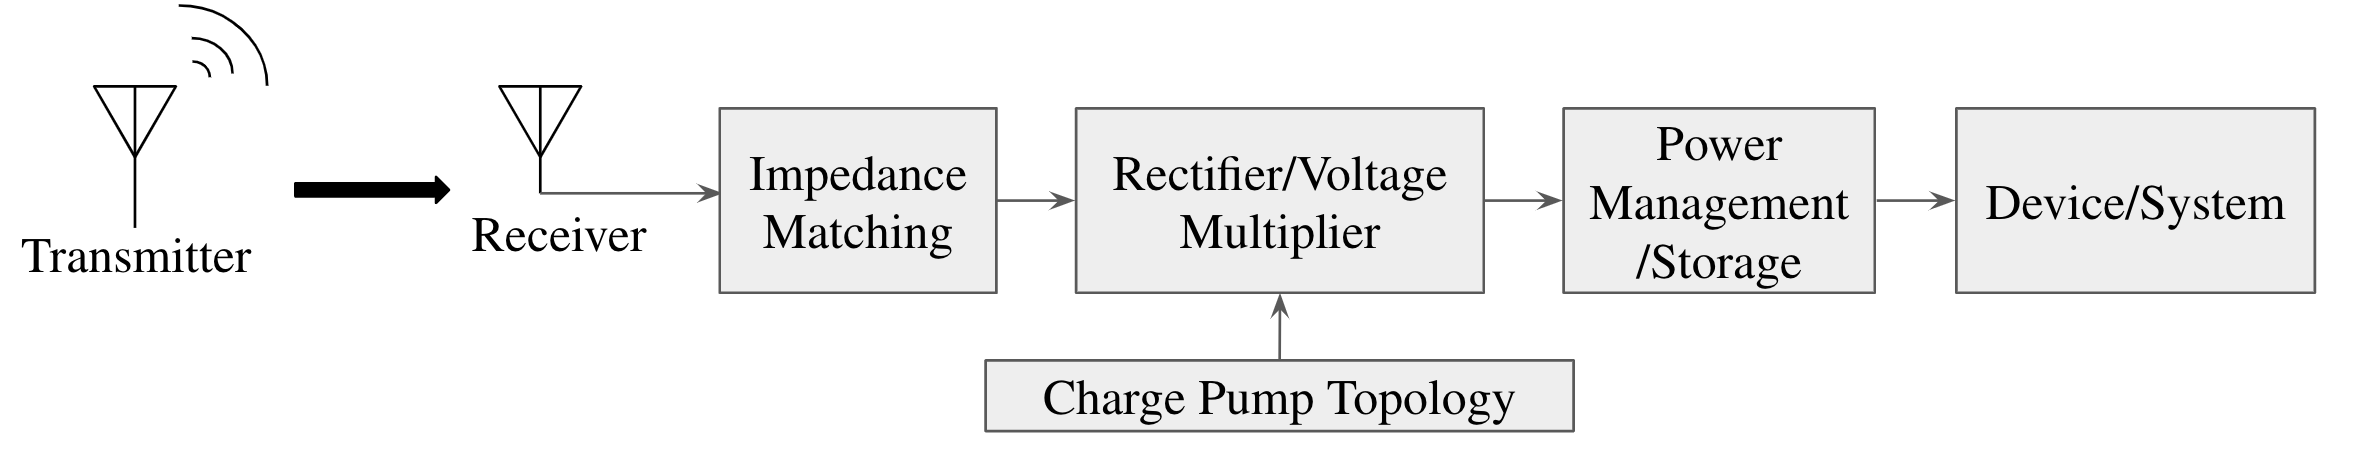
\includegraphics[scale=0.3]{ProjectPropFigure/EnergyHarvestSystem.png}}
\caption{Typical Energy Harvesting System}
\label{fig:energyharvestsystem}
\end{figure}

\noindent A full energy harvesting system starts at the transmitted RF signal generation which is then picked up by a receiver. Then some sort of impedance matching is done to deliver maximum power to the rectifier/voltage multiplier portion of the system. Eventually the power is delivered to a power management or storage system, which is used by the device or system. This project will be looking specifically at how the charge pump topology can be applied to the rectifier/voltage multiplier portion of the system. 

\subsection{Dickson Charge Pump}
In order to use energy harvesting methods as a power supply, the harvested signal needs to be boosted to a higher voltage level through a rectifier or voltage multiplier. This is because the harvested RF signal power is often insufficient to generate the necessary DC voltage level to drive a chip or sensor. The Dickson charge pump is a popular choice for low power wireless systems due to its capability of voltage multiplication. An example of the Dickson charge pump topology is depicted in Figure~\ref{fig:DicksonCP}.
	
\begin{figure}[H]
\centering{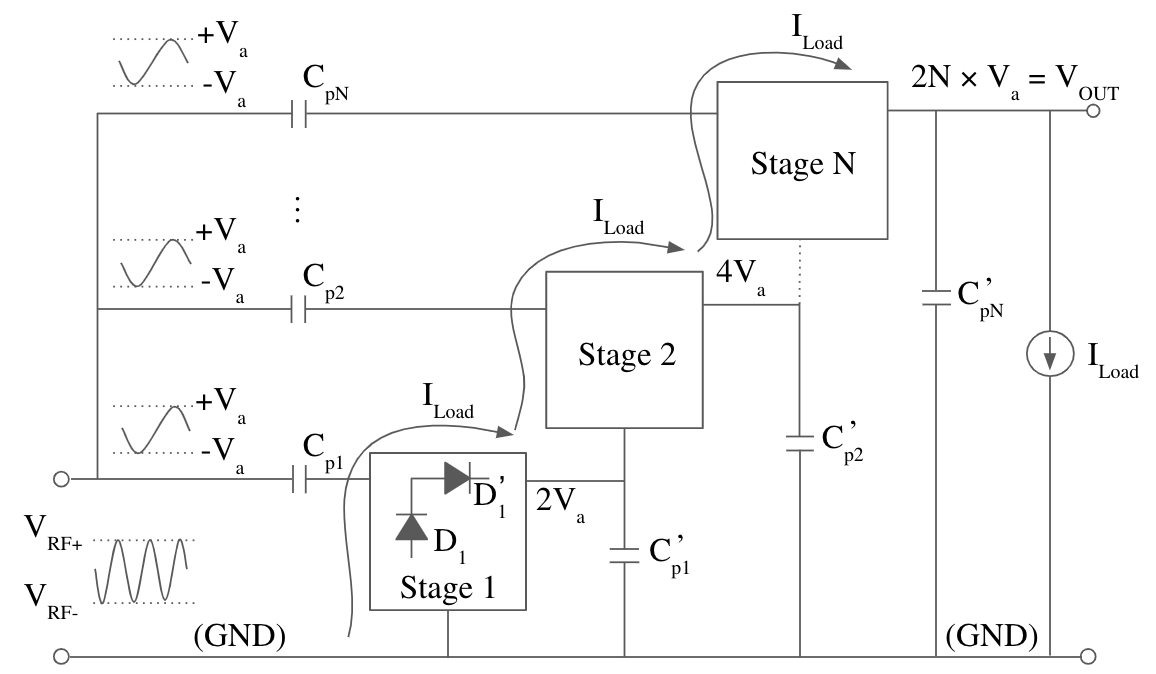
\includegraphics[scale=0.5]{ProjectPropFigure/DicksonBlock.png}}
\caption{Dickson Charge Pump \cite{Guler}}
\label{fig:DicksonCP}
\end{figure}

\noindent The basis of the working charge pump is the switching device. Figure~\ref{fig:DicksonCP} shows diodes in each stage as a passive switching device. The positive half-cycle of the signal will charge capacitors $C^{'}_{pn}$, when the negative half-cycle is reached the capacitors $C^{'}_{pn}$ are unable to discharge due to the diode orientation. As the negative half-cycle of the signal is reached, the capacitors $C_{pn}$ are charged and are unable to discharge on the positive half-cycle of the signal due to the diode orientation. Because the cascading capacitors are being utilized as storage elements a charge is accumulated in the load capacitor, however, the accumulation has diminishing returns and eventually reaches a steady state DC voltage level.\\

\subsection{Problem Statement}
Due to the low turn on voltage of Schottky diodes, they are a popular choice in charge pump designs. Other switches have been used such as MOS transistors, and will be investigated during the research stage of the project. Power efficiencies will need to be measured to determine an understanding of the most effective circuit topology.

\section{Project Description}
Charge pumps have been originally designed for use at low frequencies, however, research suggests the charge pump topology can be designed for use in the RF range to eventually be used in an energy harvester system. A closer look at the full system that will be examined in this project is shown in Figure~\ref{fig:HighLevel}.
	
\begin{figure}[H]
\centering{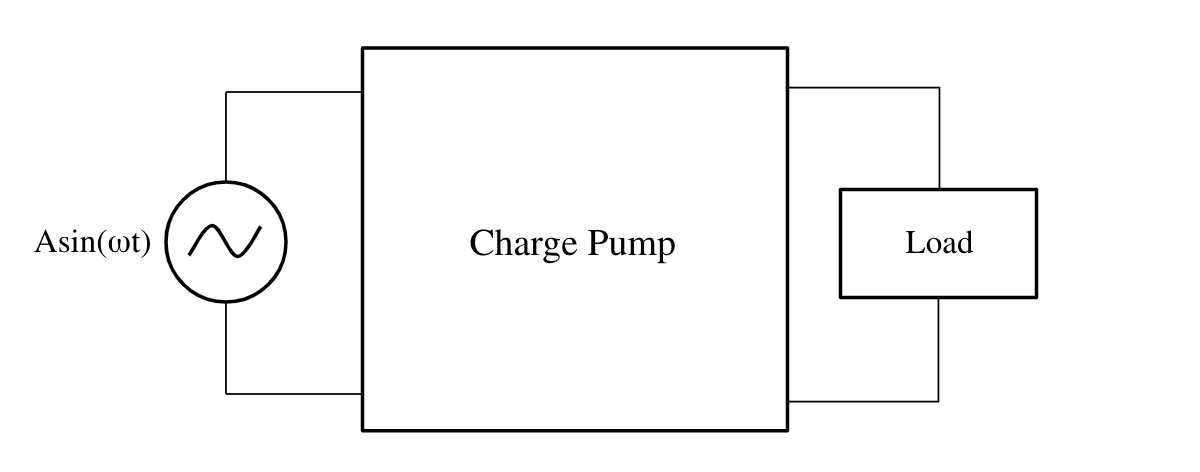
\includegraphics[scale=0.5]{ProjectPropFigure/HighLevelBlock.png}}
\caption{High Level Block Diagram}
\label{fig:HighLevel}
\end{figure}
	
\noindent A sinusoidal signal will be input directly into the charge pump block from a signal generator. The signal will then be converted to a DC voltage and dumped into a load. The signal frequency that will be used will be less than 100kHz in order to perform analysis in the time domain with the hope of scaling up to RF. \\

\noindent All RF-DC charge pumps use capacitors as storage elements in stages and many attempts to optimize the selection of components used for the charge pump have been made. Design criteria for selecting capacitor values, number of stages, and diodes in order to optimize the performance of the charge pump is the goal of this project. Multiple papers exist documenting the progress that has been made in RF-DC devices. however, further investigation is needed for improving the efficiency of power conversion, as well as possible circuit topologies, and device implementations. 
	
	\section{Review of Design}
	Charge pumps are used to passively collect RF energy signals and produce a DC output. The DC output is obtained by the capacitors cyclically charging and discharging depending on the state of a few diodes. Several characteristics must be considered when designing a charge pump circuit. The minimum voltage amplitude determined from the load current and output voltage is referred to as the sensitivity of the circuit. The sensitivity is one of the more important metrics to consider when designing the charge pump because it indicates the minimum power necessary at the input of the charge pump that will supply a DC voltage to the periodic load. Two other important metrics to consider are the power conversion efficiency~(PCE) and the voltage conversion efficiency~(VCE) given in equations 1.0 and 1.1~(pages 4 and 5). Balance between sensitivity and PCE must be made because minimizing power loss improves PCE, but higher sensitivity may degrade the PCE.  Power Efficiency~(PE) is a metric regarding power delivered to the load to power supplied at the receiver. PE and PCE can be the same if there is no impedance matching or components before the charge pump.  If impedance matching is used Power Transfer Efficiency~(PTE) which is the amount of AC power at the receiver to the power at the transmitter inductor. The sensitivity, PCE, VCE, and PE are all metrics to be considered when choosing the topology used. Dickson multiplier topology is the most common topology used. Cross-coupled multiplier topology is another option used to reduce both reverse leakage and the on-resistance of transistors.
	
	\section{Project Plan}
	The purpose of this project is to have a functioning RF energy harvesting device on a printed circuit board~(PCB). The project will result in providing research for more effective topologies and components used to produce a low voltage DC output. The three main stages of the project will include research, simulation, design, and implementation on a PCB. While the idea is to convert RF frequencies~(greater than 500MHz) to DC, experimentally we will use less than 1~MHz to get an accurate time domain response. After implementing to a PCB tests will run up to the MHz range. The functional requirements for the project are listed below:\\
	
\noindent{Functional Requirements}
\begin{itemize}
	\item Convert RF signal input to a DC signal output
	\item Maximize steady state DC output
	\item Explore different charge pump designs
	\item Design and print circuit board for testing purposes
\end{itemize}
	
	\subsection{Research}
	Research papers exploring different energy harvesting devices that include block diagrams, functional designs, and power efficiency equations have been provided. A research paper titled ``Power Management in Wireless Power-Sipping Devices: A Survey,” by Ulkuhan Guler and Maysam Ghovanloo \cite{Guler}, provides a good starting point for an understanding of the task at hand. The paper will be used as a basis for simulation of different charge pump topologies. Other research papers that will prove useful to the development of the RF-DC charge pump have been listed in the \textit{Bibliography} section on page~\pageref{bibliography}.\\
	
	\noindent “Power Management in Wireless Power-Sipping Devices: A Survey,” explains the different types of devices that can be used to construct a charge pump. The three main topologies that exist are the Greinacher Multiplier, the Dickson Multiplier, and the Cross-Coupled Multiplier. Depending on the topology that is being constructed the components can change to increase the Power Conversion Efficiency~(PCE). PCE is the ratio of DC power delivered to the load, to the AC power delivered to the input. The equation is given as follows:\footnote{Detailed explanation of equation 1 can be found in \cite{Guler}}
	
\begin{equation}
PCE = \frac{P_{Out}}{P_{In}} = \frac{P_{Out}}{P_{Out} + P_{In}}\label{eq:PCE}
\end{equation}
\vspace{1em}
\\
The voltage conversion efficiency (VCE) is the ratio between the peak voltage available at the input of the device and the DC voltage available at the output. The equation is given as follows:\footnote{Detailed explanation of equation 1 can be found in \cite{Guler}}

\begin{equation}
VCE = \frac{DC Output Voltage}{RF Peak Voltage} = \frac{V_{Out}}{V_{P}}\label{eq:VCE}
\end{equation}
\\
	The PCE and VCE equations can be used to compare the efficiency variability in the different designs that will be simulated. PCE and VCE can be optimized by carefully selecting the parts used in the charge pump. Three of the main switching devices used are Schottky diodes, diode-connected transistors, and ultra-low power diodes. Deciding which of these devices to use is based on factors such as the reverse leakage, forward loss, and availability in standard CMOS processes. Lower levels of reverse leakage improve the PCE of the device which is a big deciding factor in choosing switching devices.
	
\begin{equation}
V_{out} = 2\times N\times V_{in} - (2\times N + 1)\times V_{th}
\end{equation}

\begin{equation}
V_{out} = (V_{in} - V_{th})(\frac{C_p}{C_{par}})\times N - \frac{I_{LOAD}N}{C_pf}
\end{equation}

\begin{equation}
V_{out} = (N + 1)(V_{in} - V_{th})
\end{equation}

\begin{equation}
N = 2(\frac{V_O}{V_{in}-V_{th}}-1)
\end{equation}

\begin{equation}
C > \frac{N}{fF(N+1)^2R_{EH}}
\end{equation}
	
	\subsection{Design/Simulation}
	Simulations of the charge pump will be done using ORCAD PSpice. The simulation process will start by designing a single stage charge pump in PSpice. The starting design will be based on the standard Dickson charge pump with 1uF capacitors and Schottky diodes. The input signal will start at 1KHz with the results being gathered in the time domain.\\
	
	\noindent After analysis of the one stage charge pump response, various topologies will be created for analysis consisting of different numbers of stages, and different capacitor values. Stages will continue to be added until a three stage charge pump is created. The time domain response will be recorded from all three designs, and then be compared. The most effective design with the best PCE and VCE values~(equations~\ref{eq:PCE}~and~\ref{eq:VCE} on pages~\pageref{eq:PCE} and~\pageref{eq:VCE}) will be selected from the three designs. After selecting the design the values of the capacitors will be varied. Simulations will be run in the time domain to analyze the effect of varying values. Next, different topologies will be explored to see if the design can be further improved. A high level block diagram of the energy harvester to be designed is shown in Figure~\ref{fig:HighLevel} on page~\pageref{fig:HighLevel}.\\

\noindent The high level block diagram shows the overarching design of the energy harvester. Only the charge pump, a sinusoidal input, and a load are necessary to represent the system. The underlying charge pump block can be varied through different suggested topologies. Figure~\ref{fig:DicksonCP}  on page~\pageref{fig:DicksonCP} shows the circuit topology that will be used for a majority of the simulation and design stages.

	\subsection{Implementation}
	Once the simulations have been completed, a board design can be created for testing purposes. Prototyping will be done using breadboards and components in the lab. Once verified, a board will be designed and sent to an outside board printing company. The PCB will then be populated with components selected to our specification for testing purposes.
	
	\section{Analysis and Simulation}
	
	\subsection{Current Progress}
Analysis of the Bat68 Diode turn on voltage was simulated in Pspice. A DC sweep has been performed with a step voltage of 1mV in order to compare the forward voltage listed on the data sheet. The simulation design is shown in Figure~\ref{fig:Bat68} on page~\pageref{fig:Bat68} with the output of the DC sweep shown in Figure~\ref{fig:Bat68sim} on page~\pageref{fig:Bat68sim}. The simulation results compare to the data sheet values of the Bat68's typical forward voltage of 318mV. These simulations are likely to be repeated to determine the diode with the lowest turn on voltage within a reasonable price range.

\begin{figure}[H]
\centering{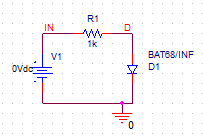
\includegraphics[scale=0.7]{ProjectPropFigure/Bat68.png}}
\caption{Bat68 Diode Analysis Model}
\label{fig:Bat68}
\end{figure}

\begin{figure}[H]
\centering{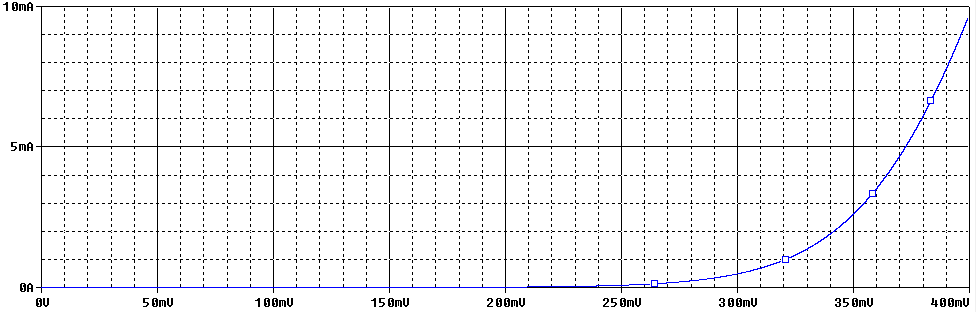
\includegraphics[scale=0.45]{ProjectPropFigure/Bat68sim.png}}
\caption{Bat68 Diode Threshold Voltage}
\label{fig:Bat68sim}
\end{figure}

\noindent Simulations of a two stage Dickson charge pump with an input amplitude of 1V with a frequency of 1kHz. The circuit was constructed using the PSpice program. Components were selected to best reflect the physical components available to build a prototype. Standard 1uF capacitors and BAT68 diodes were selected to emulate the standard capacitor values and Schottky diodes provided to build the circuit. Figure~\ref{fig:2SCP NSR} shows the layout of the designed charge pump. Time domain responses were plotted showing the voltage stepping up to a steady state. The results were recorded for 300 microseconds. Figures~\ref{fig:2SCP NSR} and~\ref{fig:2SCP NSR Out} on pages~\pageref{fig:2SCP NSR} and~\pageref{fig:2SCP NSR Out}  show the layout of the designed charge pump and the output voltage at the load resistor respectively.
	
\begin{figure}[H]
\centering{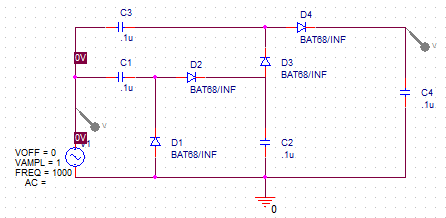
\includegraphics[scale=0.7]{ProjectPropFigure/2stageCPmodel.png}}
\caption{2-Stage Charge Pump (No Source Resistance)}
\label{fig:2SCP NSR}
\end{figure}

\begin{figure}[H]
\centering{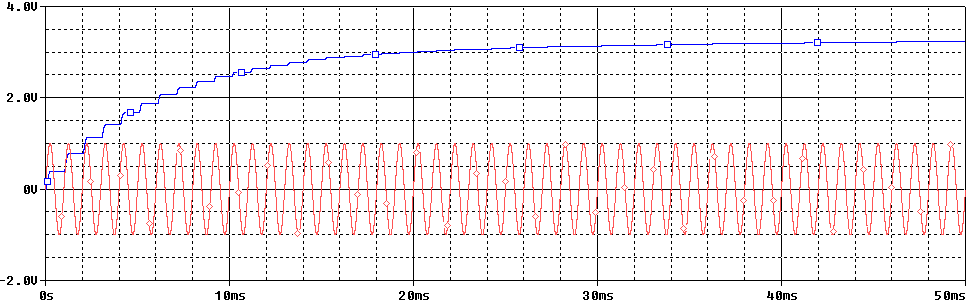
\includegraphics[scale=0.45]{ProjectPropFigure/2stageCPsim.png}}
\caption{2-Stage Charge Pump Output Voltage (No Source Resistance)}
\label{fig:2SCP NSR Out}
\end{figure}

\noindent A 50 Ohm resistor was added as a source resistance to reflect the response of a practical circuit~(see~Figure~\ref{fig:2SCP SR}). The time domain responses of the voltage was taken of the circuit and compared to the response of the circuit without the source resistance. The Simulation was run for 350 microseconds to account for the longer steady state rise time~(see~Figure~\ref{fig:2SCP SR Out}) compared to simulation shown in Figure~\ref{fig:2SCP NSR Out}.\\

\begin{figure}[H]
\centering{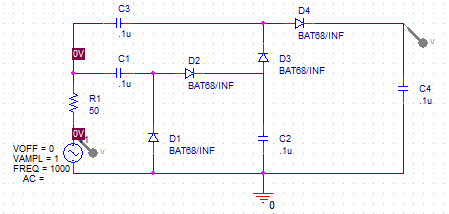
\includegraphics[scale=0.7]{ProjectPropFigure/2stageCPRmodel.png}}
\caption{2-Stage Charge Pump (With Source Resistance)}
\label{fig:2SCP SR}
\end{figure}

\begin{figure}[H]
\centering{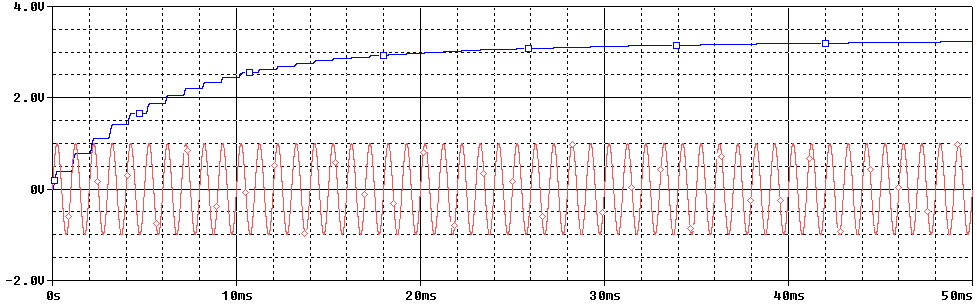
\includegraphics[scale=0.45]{ProjectPropFigure/2stageCPRsim.png}}
\caption{2-Stage Charge Pump Output Voltage (With Source Resistance)}
\label{fig:2SCP SR Out}
\end{figure}

\noindent Physical circuits of the designs were constructed to measure the response in real time. In physical circuit tests ceramic capacitors and Schottky diodes 1N5817 were provided by the labs and used. The input signal was supplied by a function generator.

\begin{figure}[H]
\centering{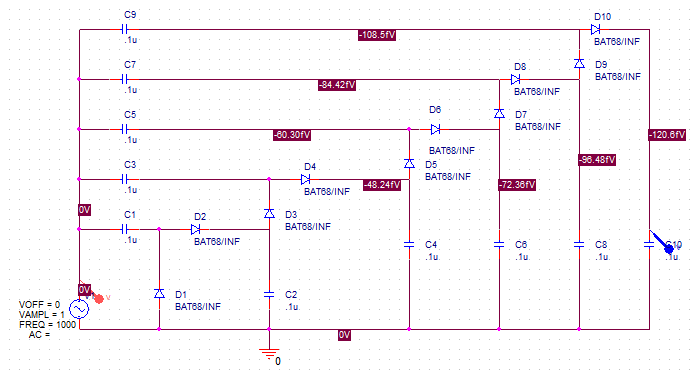
\includegraphics[scale=0.7]{ProjectPropFigure/5stageCPmodel.png}}
\caption{5-Stage Charge Pump}
\label{fig:2SCP SR}
\end{figure}

\begin{figure}[H]
\centering{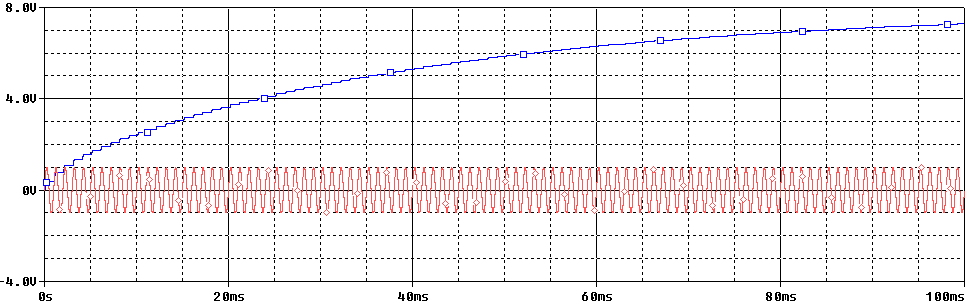
\includegraphics[scale=0.45]{ProjectPropFigure/5stageCPsim.png}}
\caption{5-Stage Charge Pump Output Voltage}
\label{fig:2SCP SR Out}
\end{figure}

ADD DESCRIPTION HERE

\begin{figure}[H]
\centering{\includegraphics[scale=0.6]{ProjectPropFigure/2stageCPLab_1kHZ_1V.png}}
\caption{2-Stage Charge Pump Lab Output}
\label{fig:2SCP SR}
\end{figure}

ADD DESCRIPTION HERE

\begin{figure}[H]
\centering{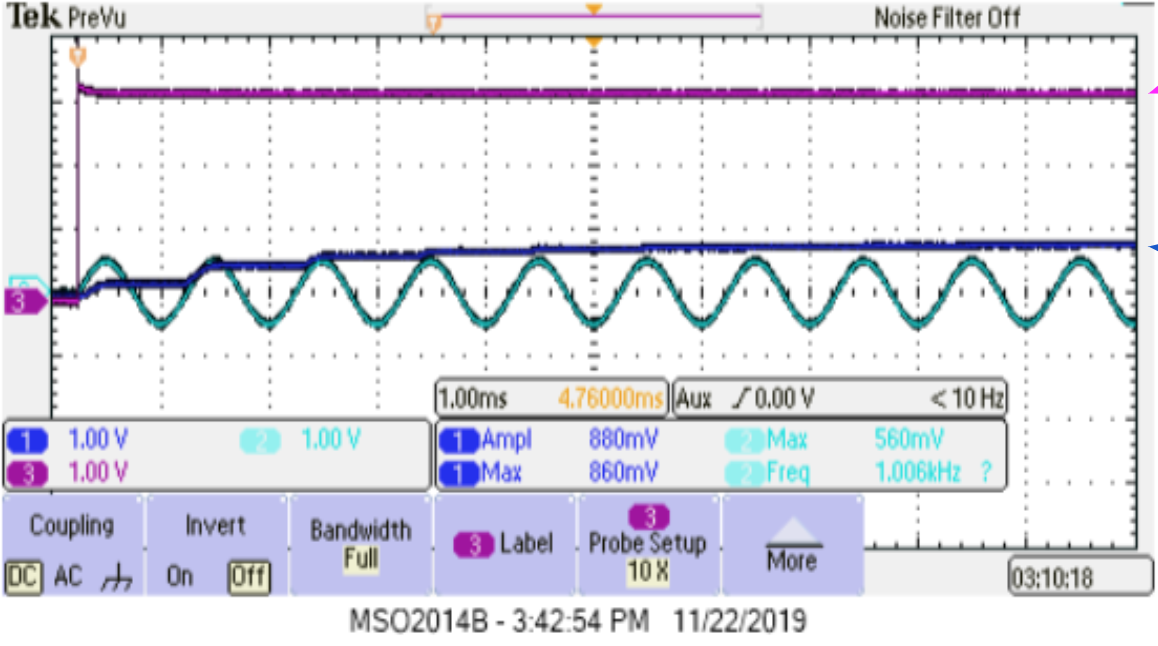
\includegraphics[scale=0.6]{ProjectPropFigure/2stageCPLab_1kHz_500mV.png}}
\caption{2-Stage Charge Pump Output Lab Output}
\label{fig:2SCP SR Out}
\end{figure}

ADD DESCRIPTION HERE

	\subsection{Future Plans}
More simulations must be performed in an effort to optimize the construction of the charge pump. Tests will be performed by varying the different number of levels in the charge pump versus the value of the capacitors to verify which causes a charge pump of charge up faster. Ideally the simulations can be performed and finished over winter break and January. Circuits will be built in the labs in February and March. An attempt to find a correlation or formulate some equation that will optimize the values of capacitors and number of levels for a charge pump will be made using the results of the simulations and physical circuit tests. By the end of March to mid April a circuit board prototype will be made. Parts to construct a PCB will need to be ordered at a later date when a method for optimization is formulated.
	
	TALK ABOUT CHANGE MODELING OF IDEAL DIODES 
	
	\section{Conclusion}
Future uses for RF-DC energy harvesting devices include any low power applications such as period measurement systems, medical sensors, space and aerospace applications, etc. The experience gained from this capstone project will transfer into hardware design and RF design. After designing and implementing to a physical circuit board a better understanding of the design process will be an important outcome. The hope is to have a published research paper at the end of the project as well as added experience.
	
	HOW WILL THIS PROJECT MAKE AN IMPACT?
	
	
	\newpage
	\label{bibliography}
	\nocite{*}
	\printbibliography
	
\end{document}